\section{Метод многих сфер для описания электростатического взаимодействия двух тел}
\label{SEC:MSM}

Метод многих сфер предназначен для аппроксимации электростатического взаимодействия между проводящими объектами произвольных форм.
Космический аппарат или космический мусор моделируется набором сфер с фиксированными размерами и относительными положениями (рис.\ref{ris:sp_msm})\cite{msm}.
Внешняя сфера используется для разрешения сил и вращающих моментов на теле для определения оптимального решения параметров модели.
Предположим далее, что оптимальные относительные положения и размеры $n$ сфер в модели уже определены.
Получившийся набор сфер должен перемещаться и вращаться как изначальное тело.
Внешнюю сферу так же можно заменить другим объектом общей формы, описанным с помощью набора заряженных сфер.
Для каждого объекта нужно определить начало отсчета. Для аппарата на рисунке \ref{ris:sp_msm} это будет точка $O$. 

\begin{figure}[H]
	\center{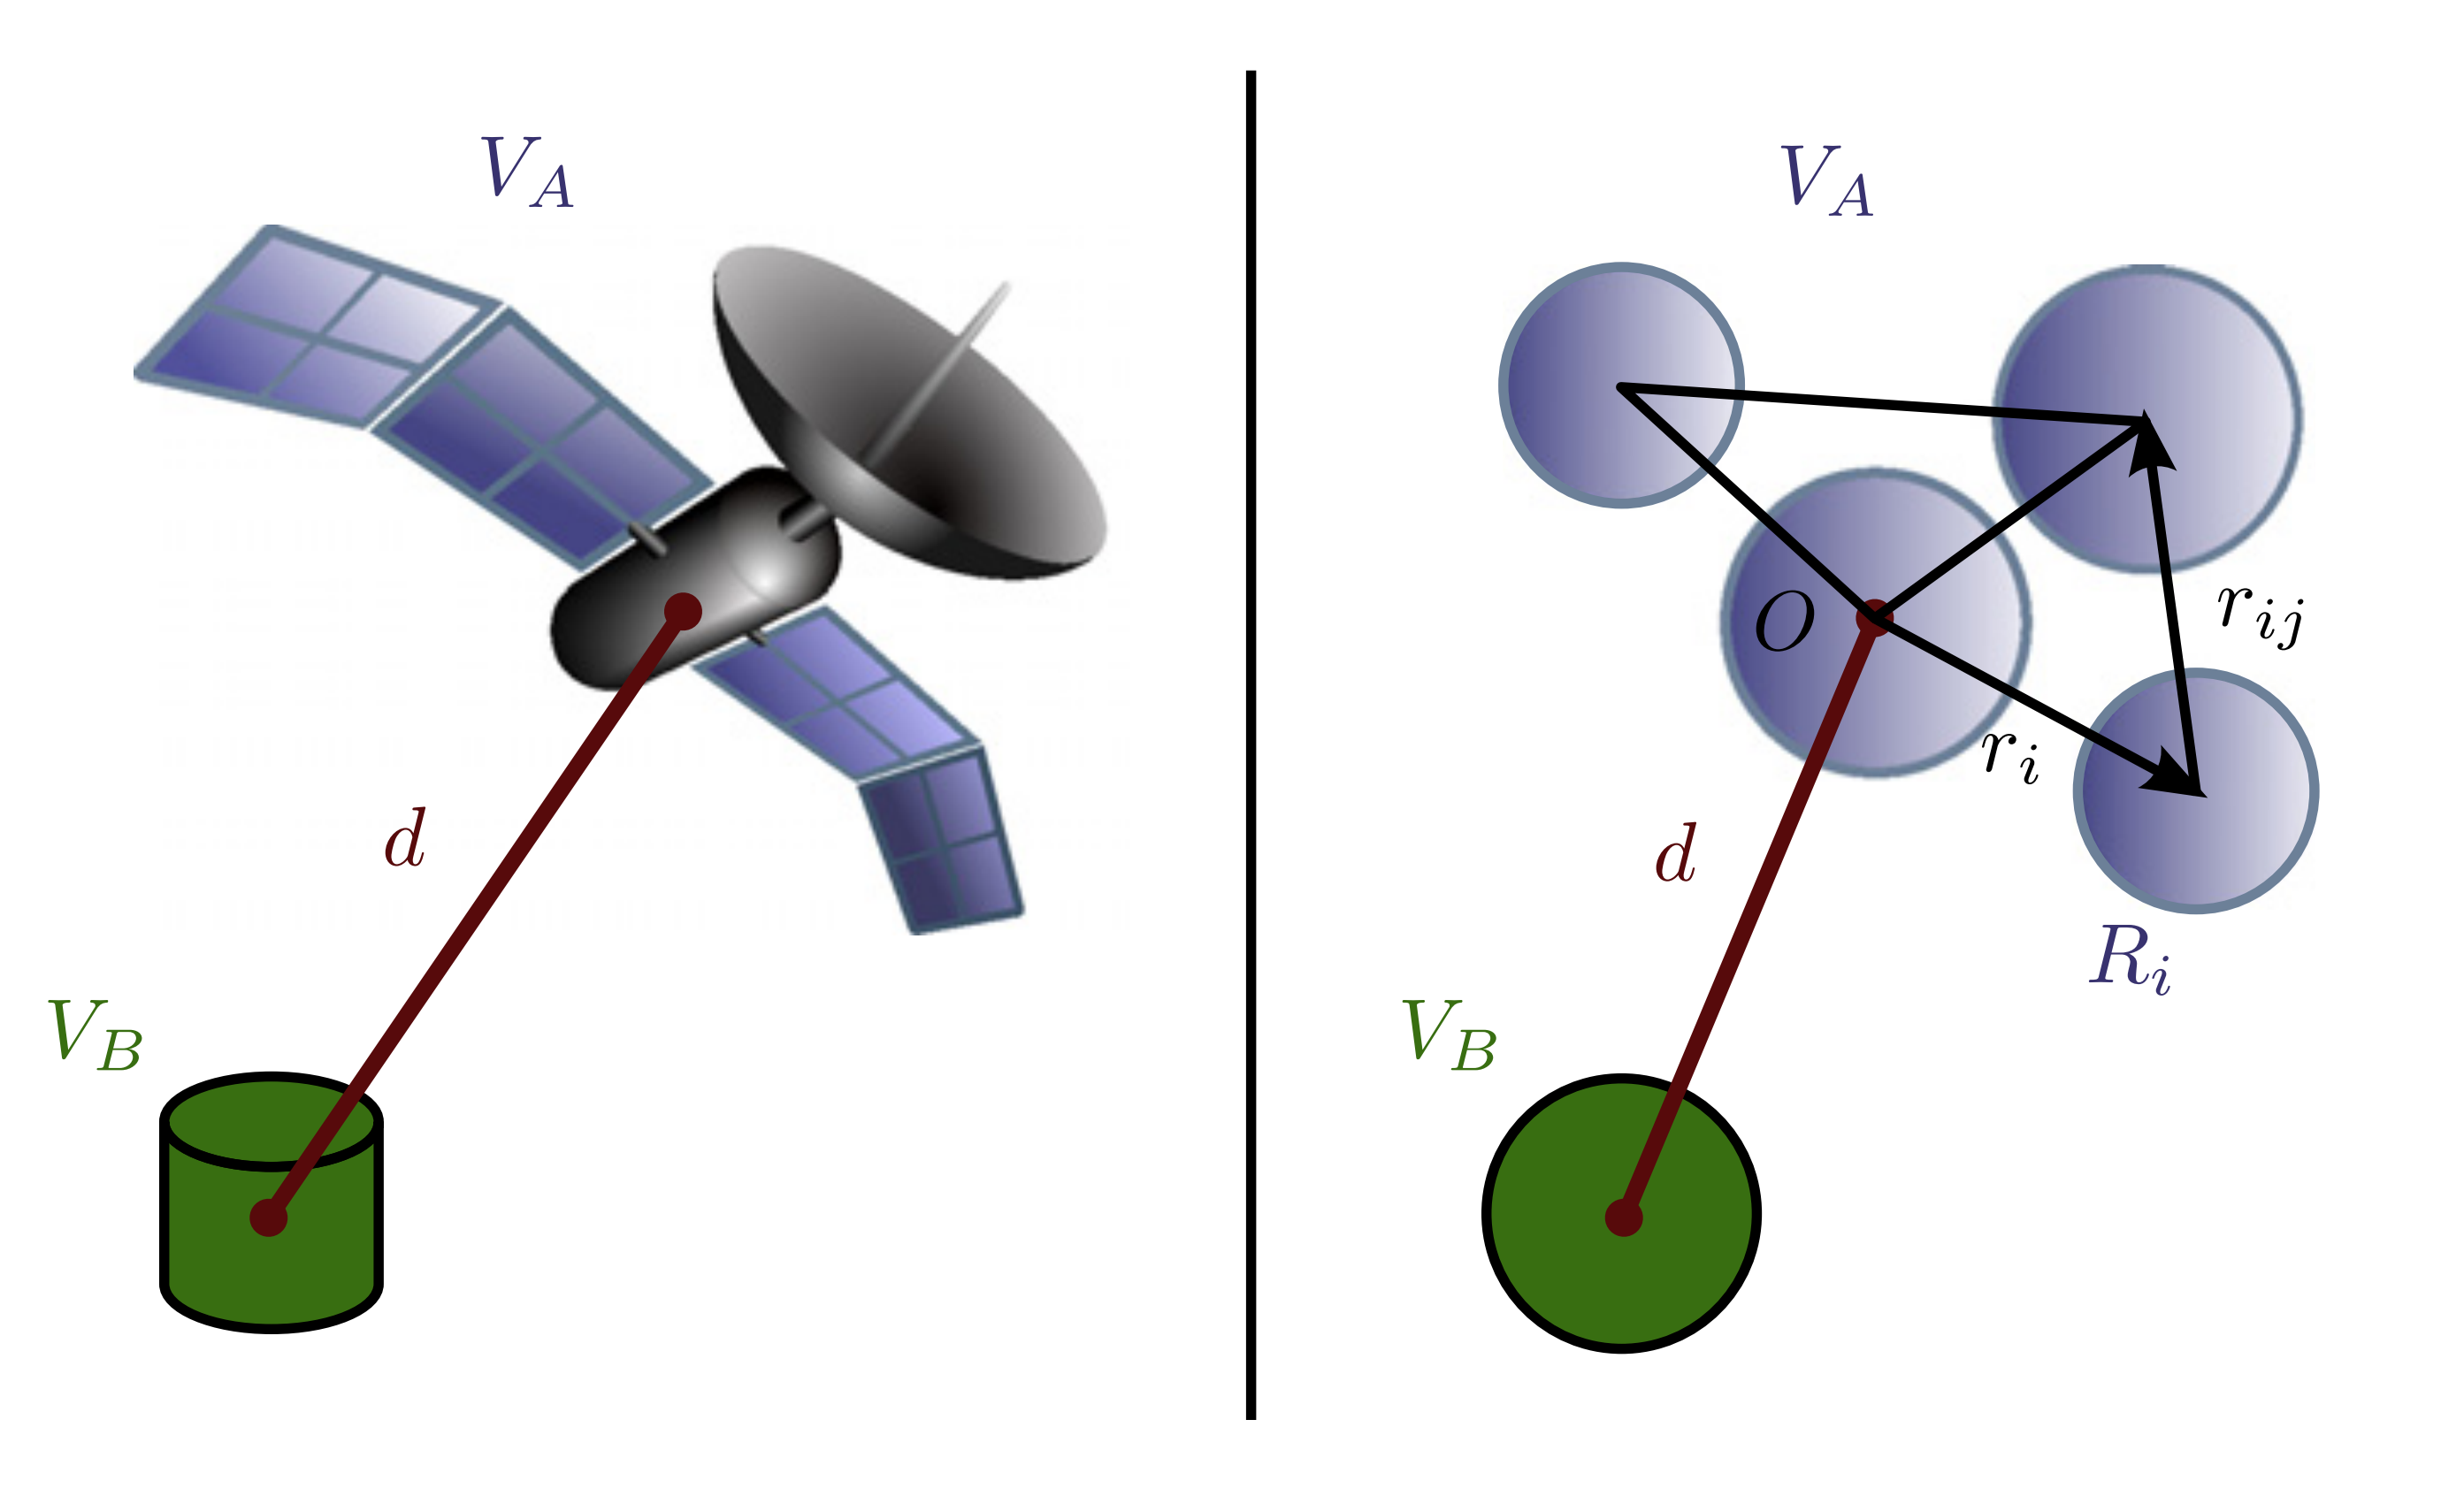
\includegraphics[scale=0.35]{spacecraft_msm.png}}
	\caption{Концептуальное описание метода многих сфер}
	\label{ris:sp_msm}
\end{figure}

Абсолютное электростатическое напряжение предполагается расположенным на космическом аппарате.
При этом кулоновская сила взаимодействия между сферами зависит от заряда каждой сферы.
Напряжение $\Phi_i$ на каждой сфере зависит как от заряда самой сферы, так и от заряда соседних с ней сфер и определяется по формуле \cite{2sph}:
\begin{equation}
\label{eq:voltage}
	\Phi_i = k_c \frac{q_i}{R_i} + \sum_{j=1,j\neq i}^{m} k_c \frac{q_j}{r_{i,j}},
\end{equation}
где $R_i$ – радиус $i$-ой сферы, $r_{i,j} = r_j - r_i$ – расстояние между центрами соседних сфер, $k_c = \frac{1}{4\pi\varepsilon_0} = 8.99 * 10^9 \frac{N*m^2}{C^2}$ – постоянная Кулона, $q_i$ – заряд $i$-ой сферы.

Линейные отношение из (\ref{eq:voltage}) для каждой из $m = n + 1$ сфер ($n$ сфер описывают тело и одна внешняя) в системе можно представить в матричном виде \cite{msm}:
\begin{equation}
\label{eq:voltage_matr}
	\vec{\Phi} = k_c [C_m]^{-1} \vec{q},
\end{equation}
где $\vec{\Phi} = [\Phi_A, \Phi_A, \dots, \Phi_A, \Phi_B]^T$ – вектор напряжений, $\vec{q} = [q_1, q_2, \dots, q_n, q_b]^T$ – вектор зарядов, $\Phi_A$ – напряжение каждой сферы тела, $\Phi_B$ – напряжение внешней сферы, $C_m$ – матрица ёмкостей, обратная матрица к которой имеет вид:
\begin{equation}
\label{eq:cm_inv}
	[C_m]^{-1} = 
	\begin{pmatrix}
		1/R_1	&	1/r_{1,2}	&	\dots		&	1/r_{1,n}	&	1/r_{1,B} \\
		1/r_{1,2}	&	1/R_1	&	\dots		&	\vdots		&	\vdots \\
		\vdots		&	\ddots		&	\ddots	&	\vdots		&	\vdots \\
		1/r_{n,1}	&	\dots			&	\dots		&	1/R_n	&	1/r_{n,B} \\
		1/r_{B,1}	&	\dots			&	\dots		&	1/r_{B,n}	&	1/R_B
	\end{pmatrix},
\end{equation}
где $\vec{r}_{i,B} = \vec{d} - \vec{r}_i$.

Далее, решив систему уравнений (\ref{eq:voltage_matr}) с помощью взятия обратной матрицы к (\ref{eq:cm_inv}), получим функции от времени для зарядов $q_i$.
Имея выражения для зарядов, можно вычислить силу взаимодействия сфер.
Тело предполагаем твёрдым, что дает нам постоянные положения сфер относительно друг друга.
Полная сила взаимодействия $F$ и вращающий момент $L_O$ для тела $A$ в точке $O$ описываются формулами (\ref{eq:force_msm}) и (\ref{eq:torque_msm}) соответственно \cite{msm}.

\begin{equation}
\label{eq:force_msm}
	\vec{F} = k_c q_B \sum_{i=1}^n \frac{q_i}{\norm{\vec{r}_{i,B}}^3}\vec{r}_{i,B}.
\end{equation}

\begin{equation}
\label{eq:torque_msm}
	\vec{L}_O = k_c q_B \sum_{i=1}^n \frac{q_i}{\norm{\vec{r}_{i,B}}^3} \vec{r}_i \times \vec{r}_{i,B}.
\end{equation}